\documentclass[spanish]{udpreport}
\usepackage[utf8]{inputenc}
\usepackage[spanish]{babel}
\usepackage{float}
\usepackage{subcaption}


% Podemos establecer el logo de alguna entidad o dejar el de la UDP (defecto)
%\setlogo{EITFI}

\title{Informe Laboratorio 5 \\ Redes de Datos}
% ** Numero del lab
\author{Arturo Mantinetti \\ Manuel Tobar \\ Diego Vilches \\ Nicolas Henriquez}
\email{arturo.mantinetti@mail.udp.cl \\ manuel.tobar@mail.udp.cl
	\\ diego.vilches@mail.udp.cl \\ nicolas.henriquez@mail.udp.cl}
	
\profesor{Profesor \\ Jaime Álvarez}
\ayudante{Ayudante \\ Maximiliano Vega}


\date{** de Julio de 2016}
% ** = Dia de entrega

% Además podemos establecer la facultad y escuela
% los valores por defecto son los siguientes:
%\udpschool{Escuela de Informática y Telecomunicaciones}
%\udpfaculty{Facultad de Ingeniería}
%\udpuniversity{Universidad Diego Portales}

\begin{document}
\maketitle

\tableofcontents

\chapter{Introducción}

Este laboratorio consistió en armar una simulación de red en Packet Tracer con distintas configuraciones dentro de la red para comprender el funcionamiento del ruteo estático y el ruteo dinámico.

\chapter{Software utilizado}
La aplicación usada en esta ocasión para simular las distintas redes sera Packet Tracer. Este programa es propiedad de Cisco y permite experimentar con el comportamiento de la red y resolver preguntas de que ocurriría con la red si realizamos cierta configuración o conexión de dispositivos.

\begin{figure}[H]
	\centering
	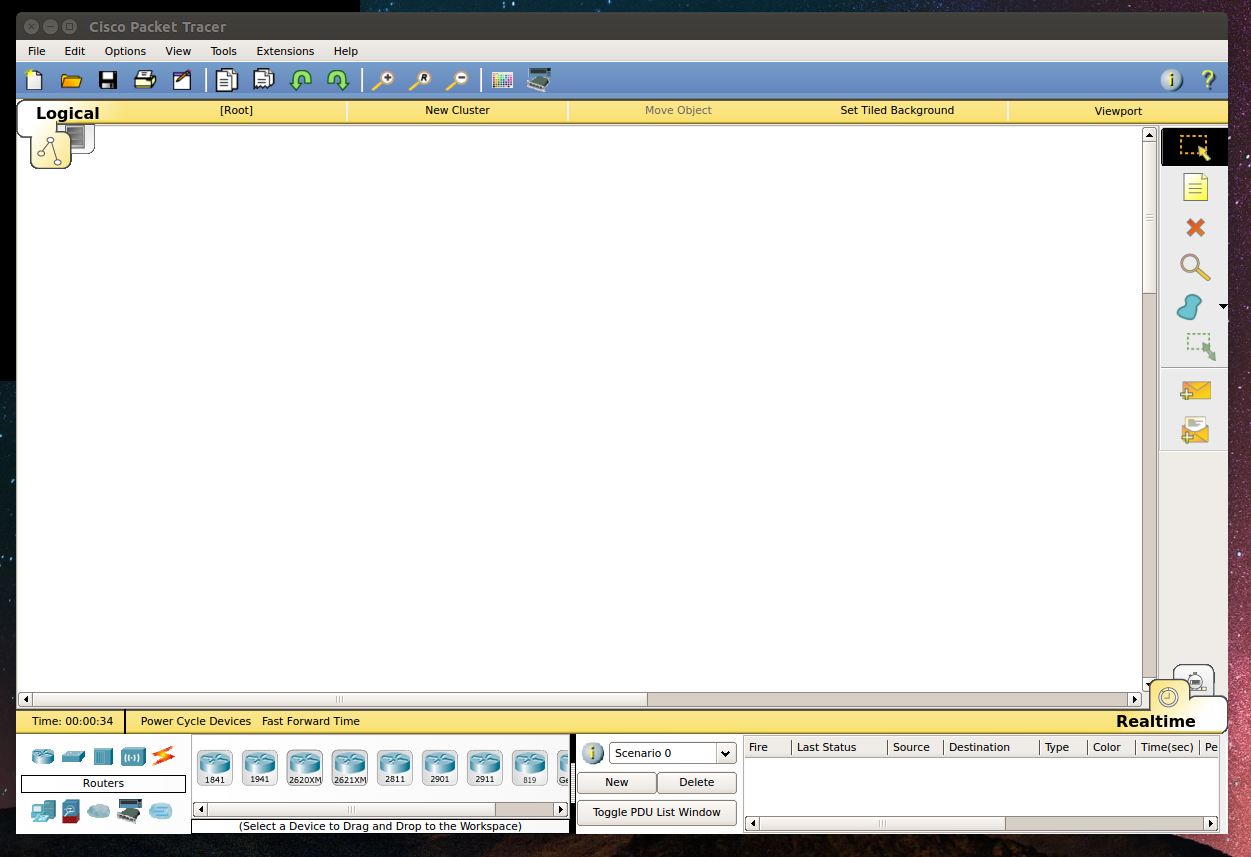
\includegraphics[scale=.25]{imagenes/A0e.png}
	\caption{Packet Tracer}
	\label{fig:Figura 1.1}
\end{figure}


\chapter{Actividades}

\section{Actividad I}

La primera actividad consiste en montar una topología tipo anillo con cuatro routers. Desde cada router una topología tipo árbol, compuesta por un switch y dos computadores cada una.

\begin{figure}[H]
	\centering
	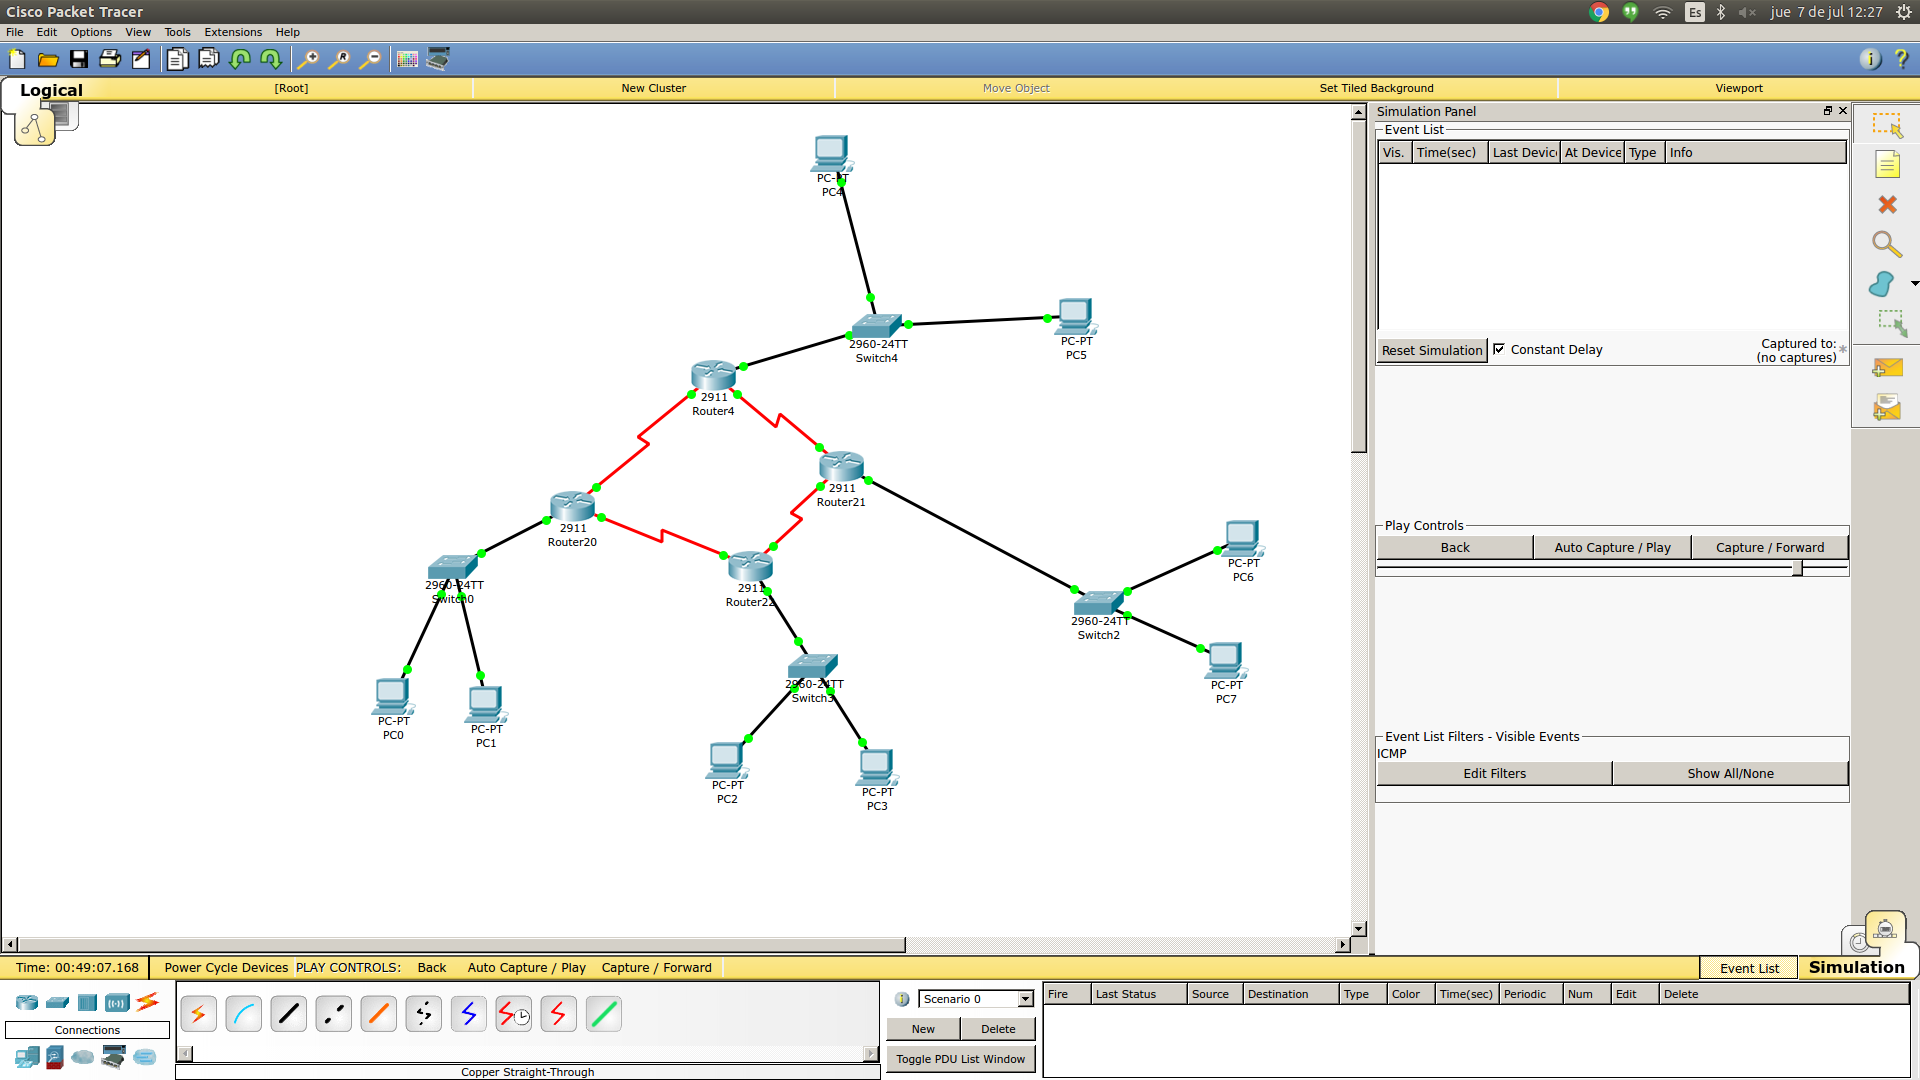
\includegraphics[scale=.25]{imagenes/red.png}
	\caption{Topología de Red}
	\label{fig:Figura 2.1}
\end{figure}

\section{Actividad II}

Esta actividad consiste en configurar los equipos con sus respectivas IP's, Mascaras y Puertas de Enlace. Cada conjunto de equipos estaba conectado a un router con una red distinta, además de que fue establecida una red distinta para los routers interconectados.

\begin{figure}[H]
	\centering
	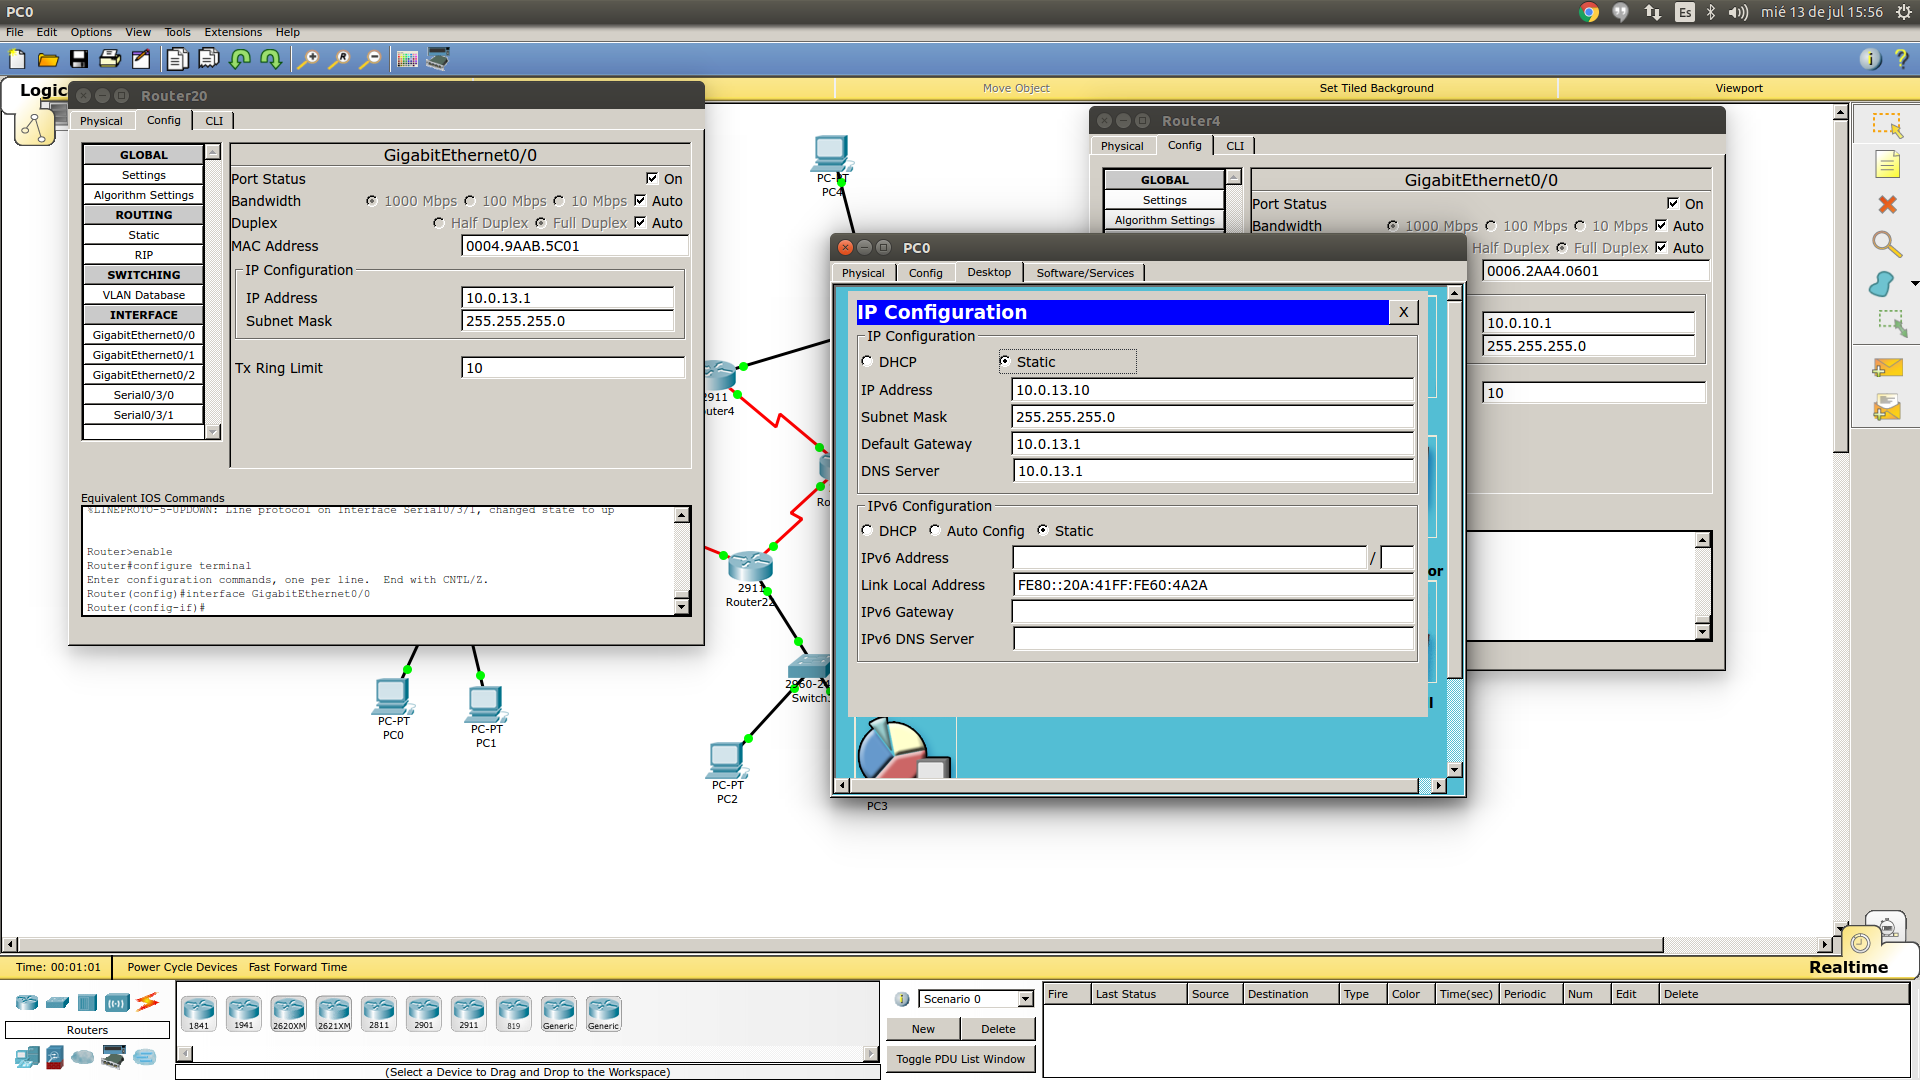
\includegraphics[scale=.25]{imagenes/ips.png}
	\caption{Configuración de Equipos}
	\label{fig:Figura 3.1}
\end{figure}


\section{Actividad III}

En esta parte del laboratorio se configuraron los rourters con ruteo estatico

\begin{figure}[H]
	\centering
	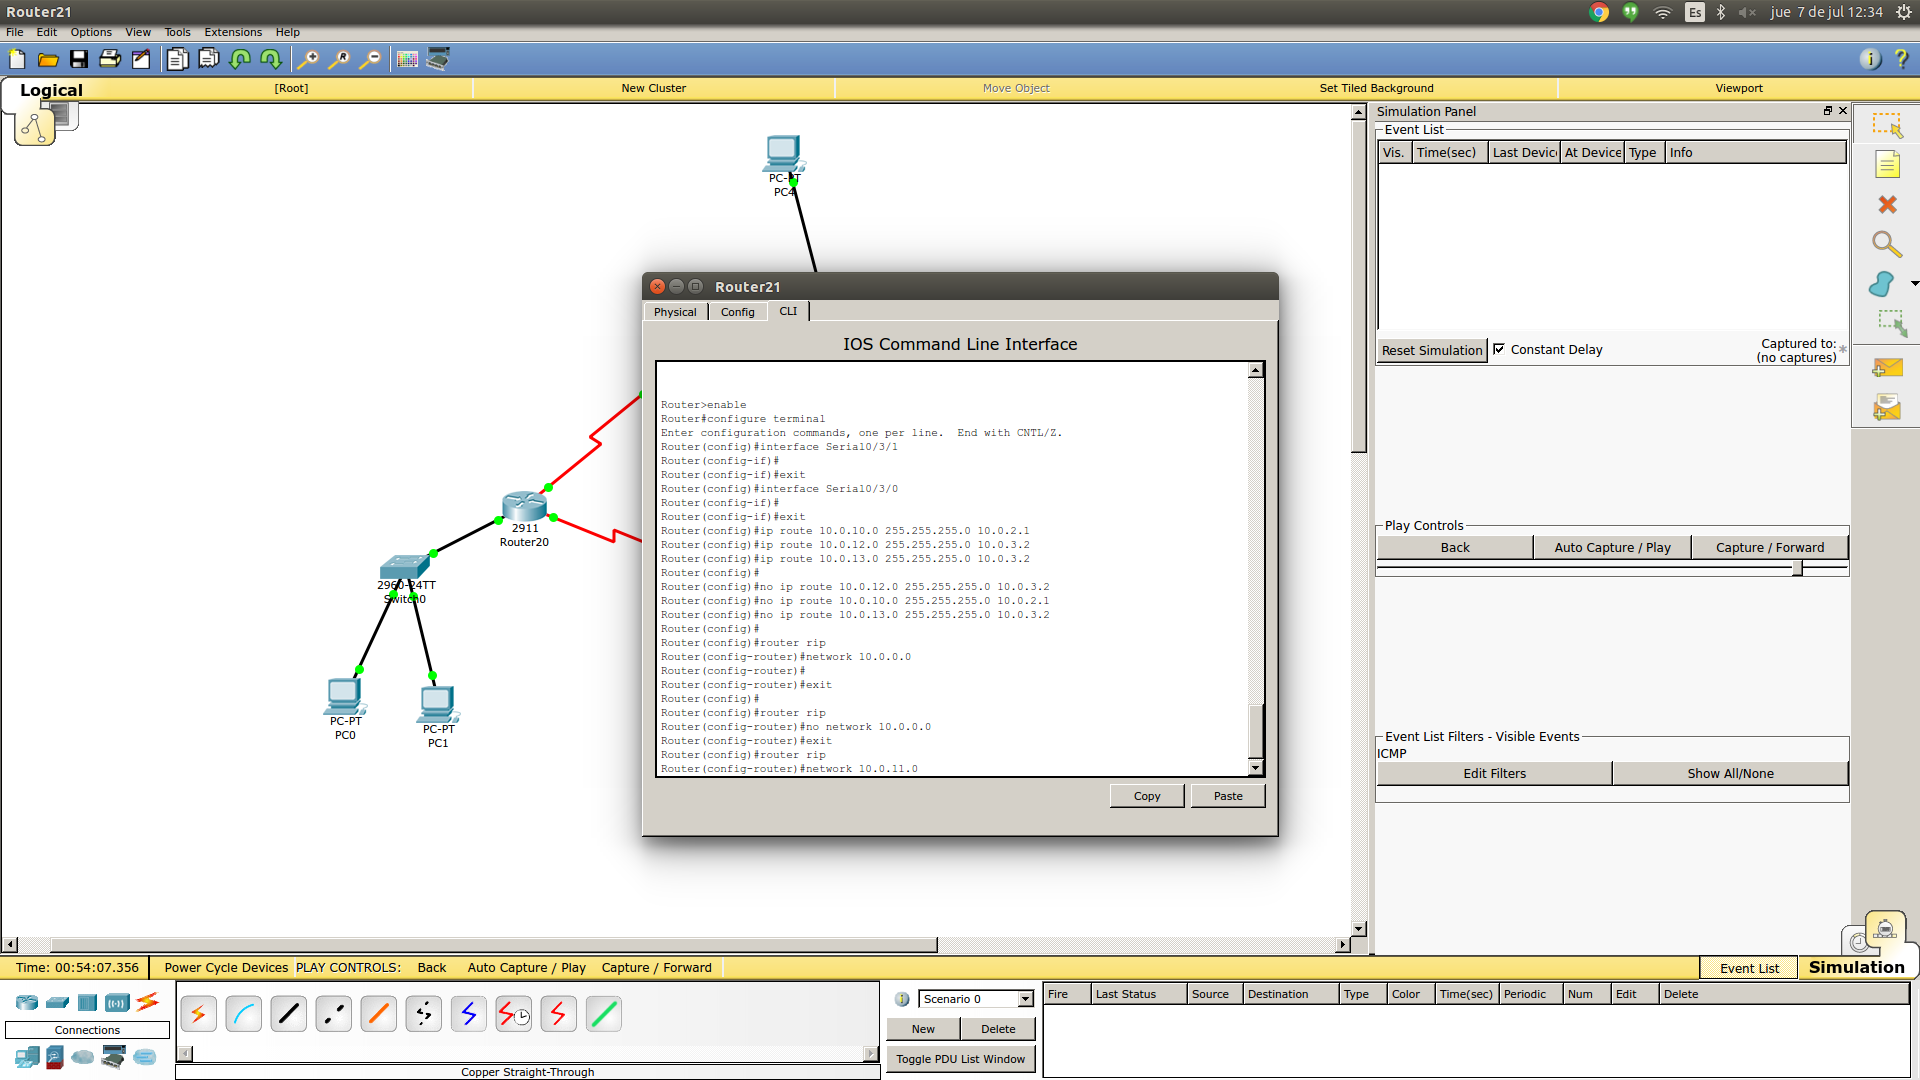
\includegraphics[scale=.25]{imagenes/ruteo_estatico.png}
	\caption{Configuración Ruteo Estático}
	\label{fig:Figura 4.1}
\end{figure}

\begin{figure}[H]
	\centering
	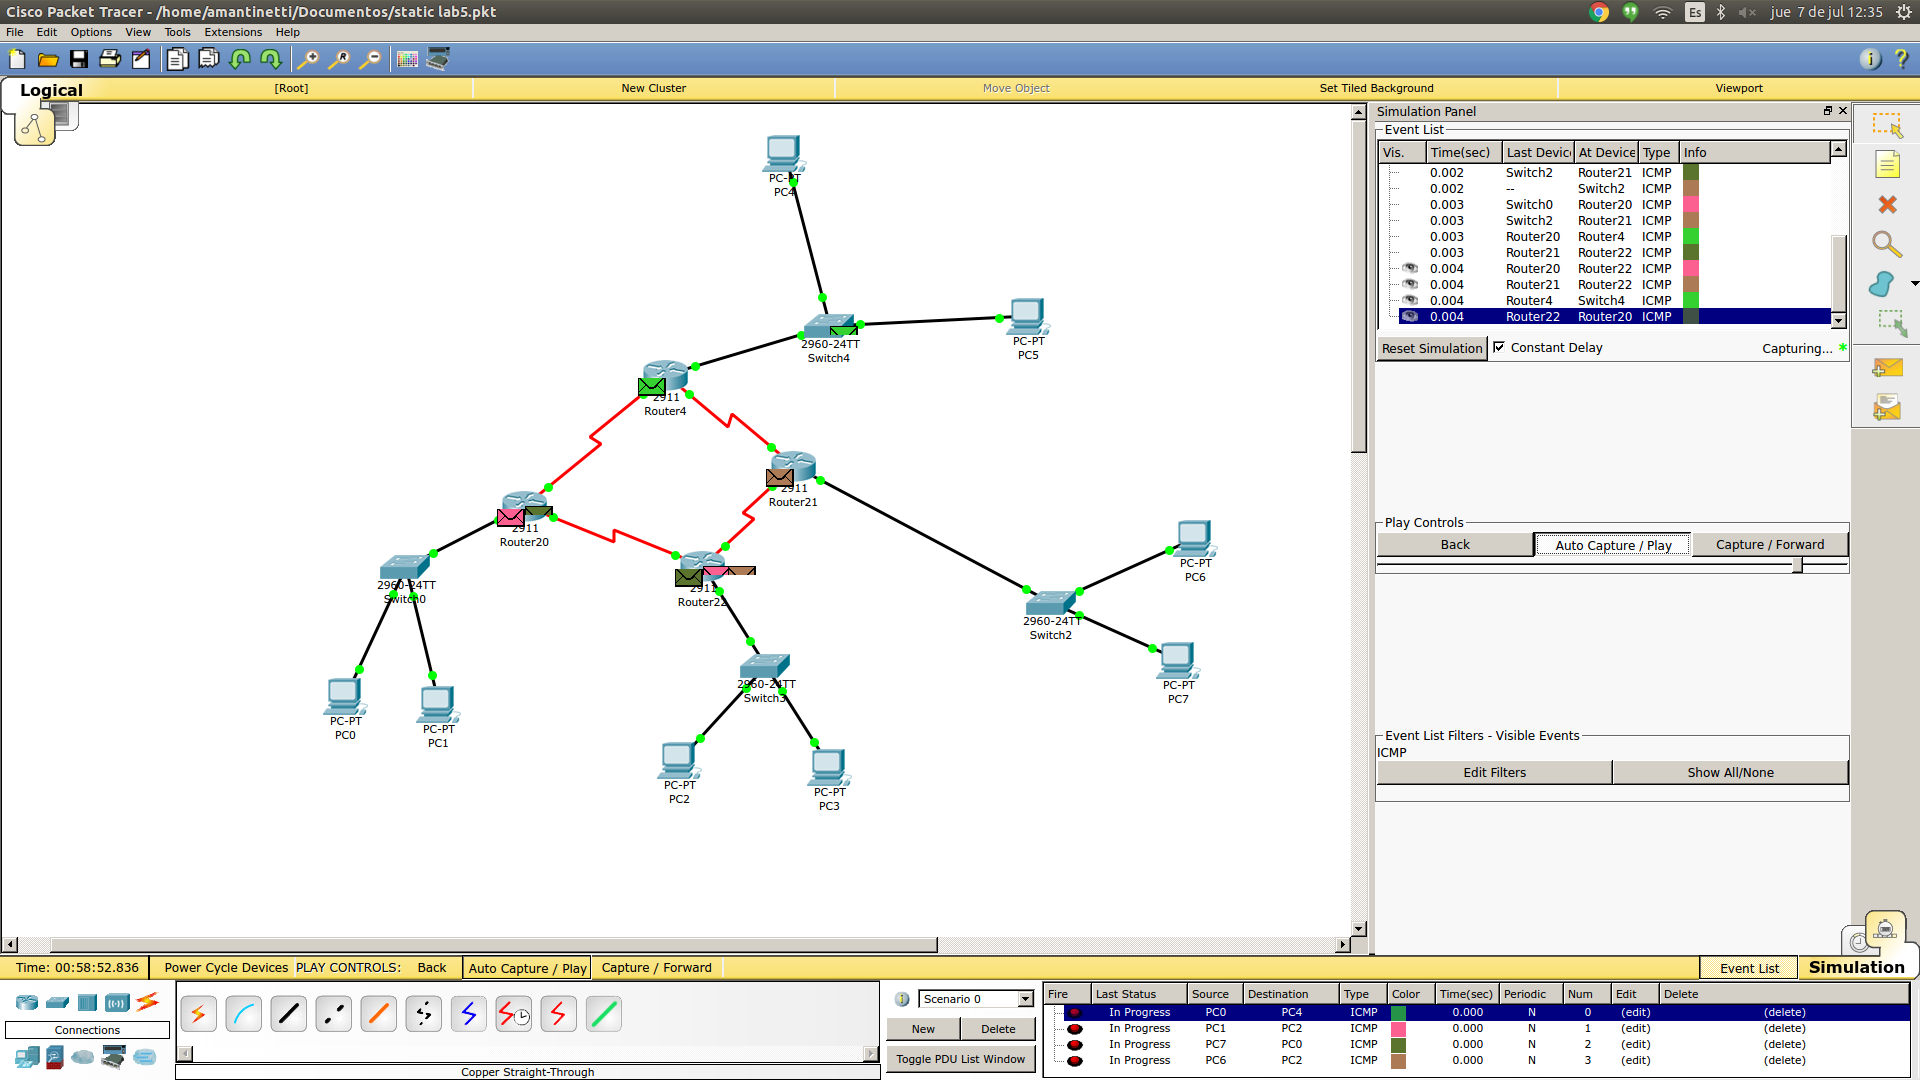
\includegraphics[scale=.25]{imagenes/test_restatico.png}
	\caption{Test Ruteo Estático}
	\label{fig:Figura 4.2}
\end{figure}

\section{Actividad IV}

Finalmente, en esta actividad del laboratorio, se configuraron los routers con ruteo dinámico

\begin{figure}[H]
	\centering
	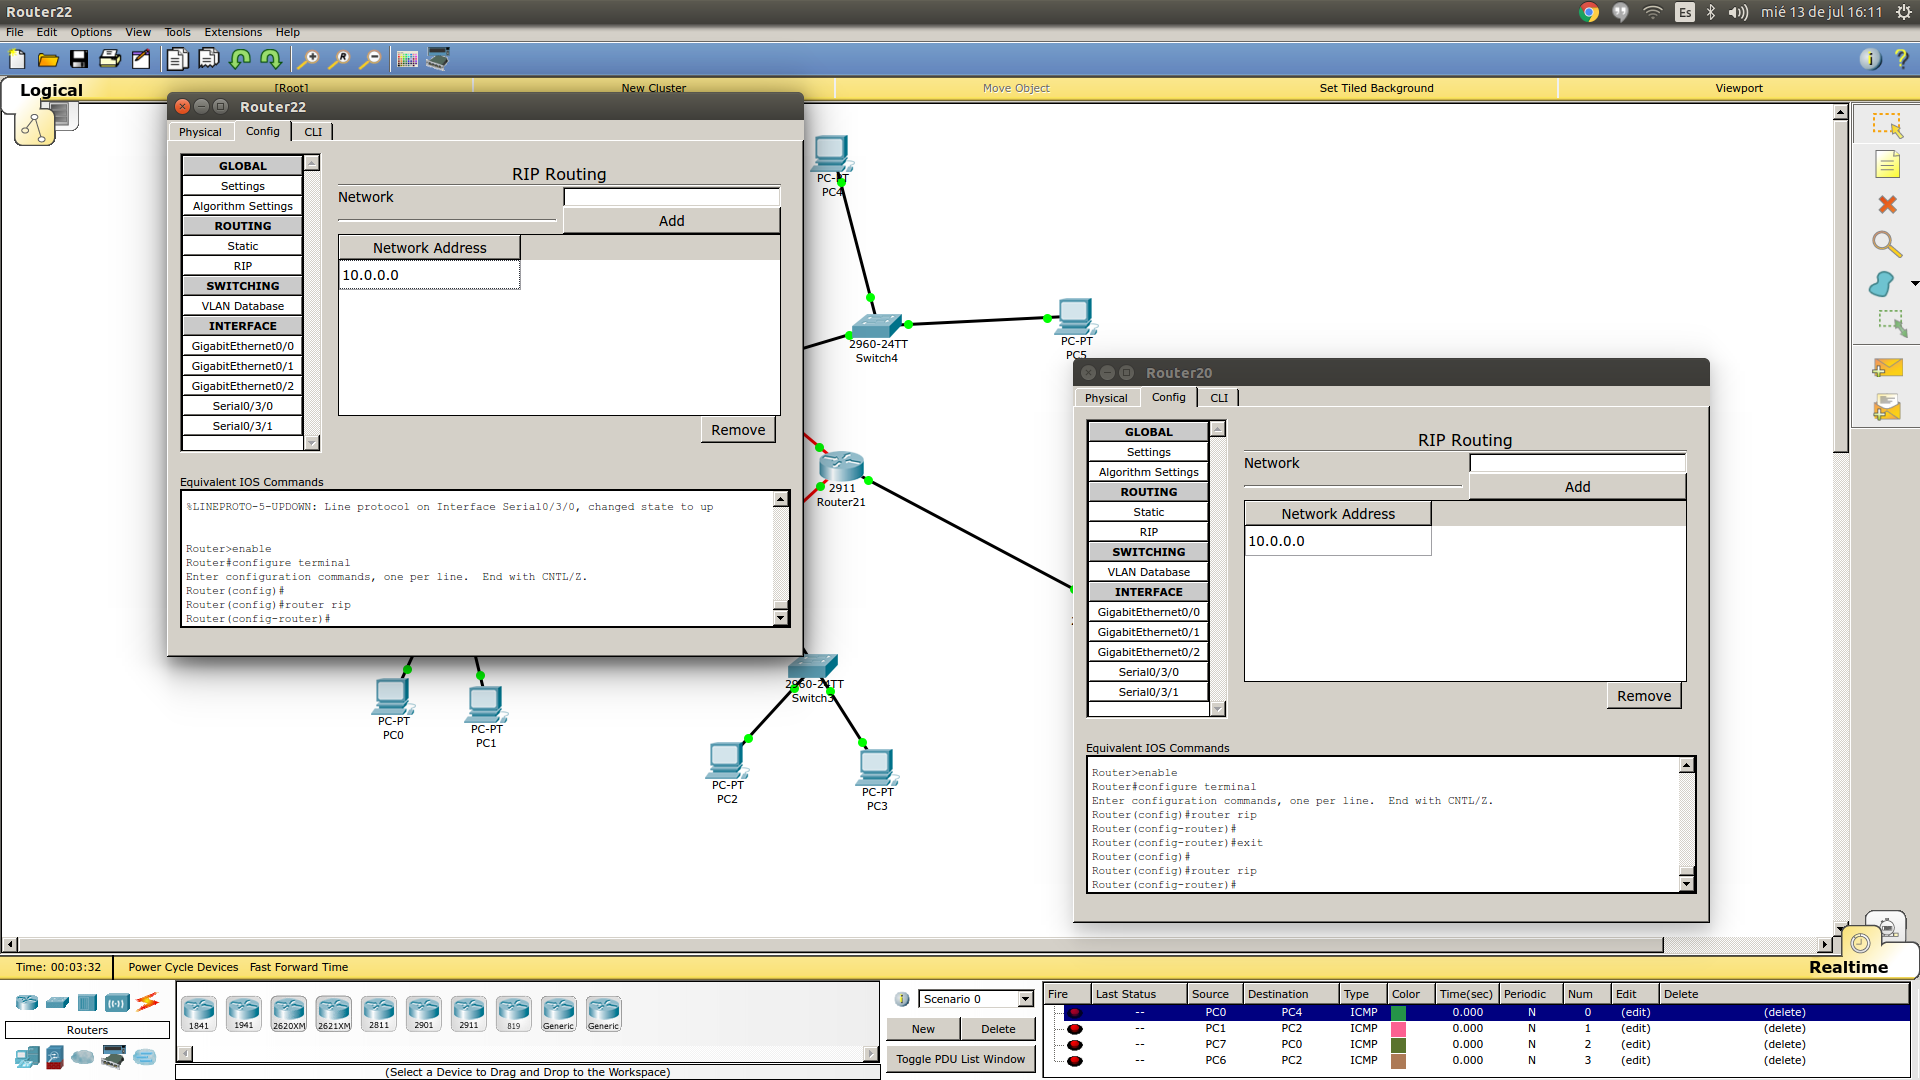
\includegraphics[scale=.25]{imagenes/ruteo_dinamic.png}
	\caption{Configuración Ruteo Dinámico}
	\label{fig:Figura 4.1}
\end{figure}

\begin{figure}[H]
	\centering
	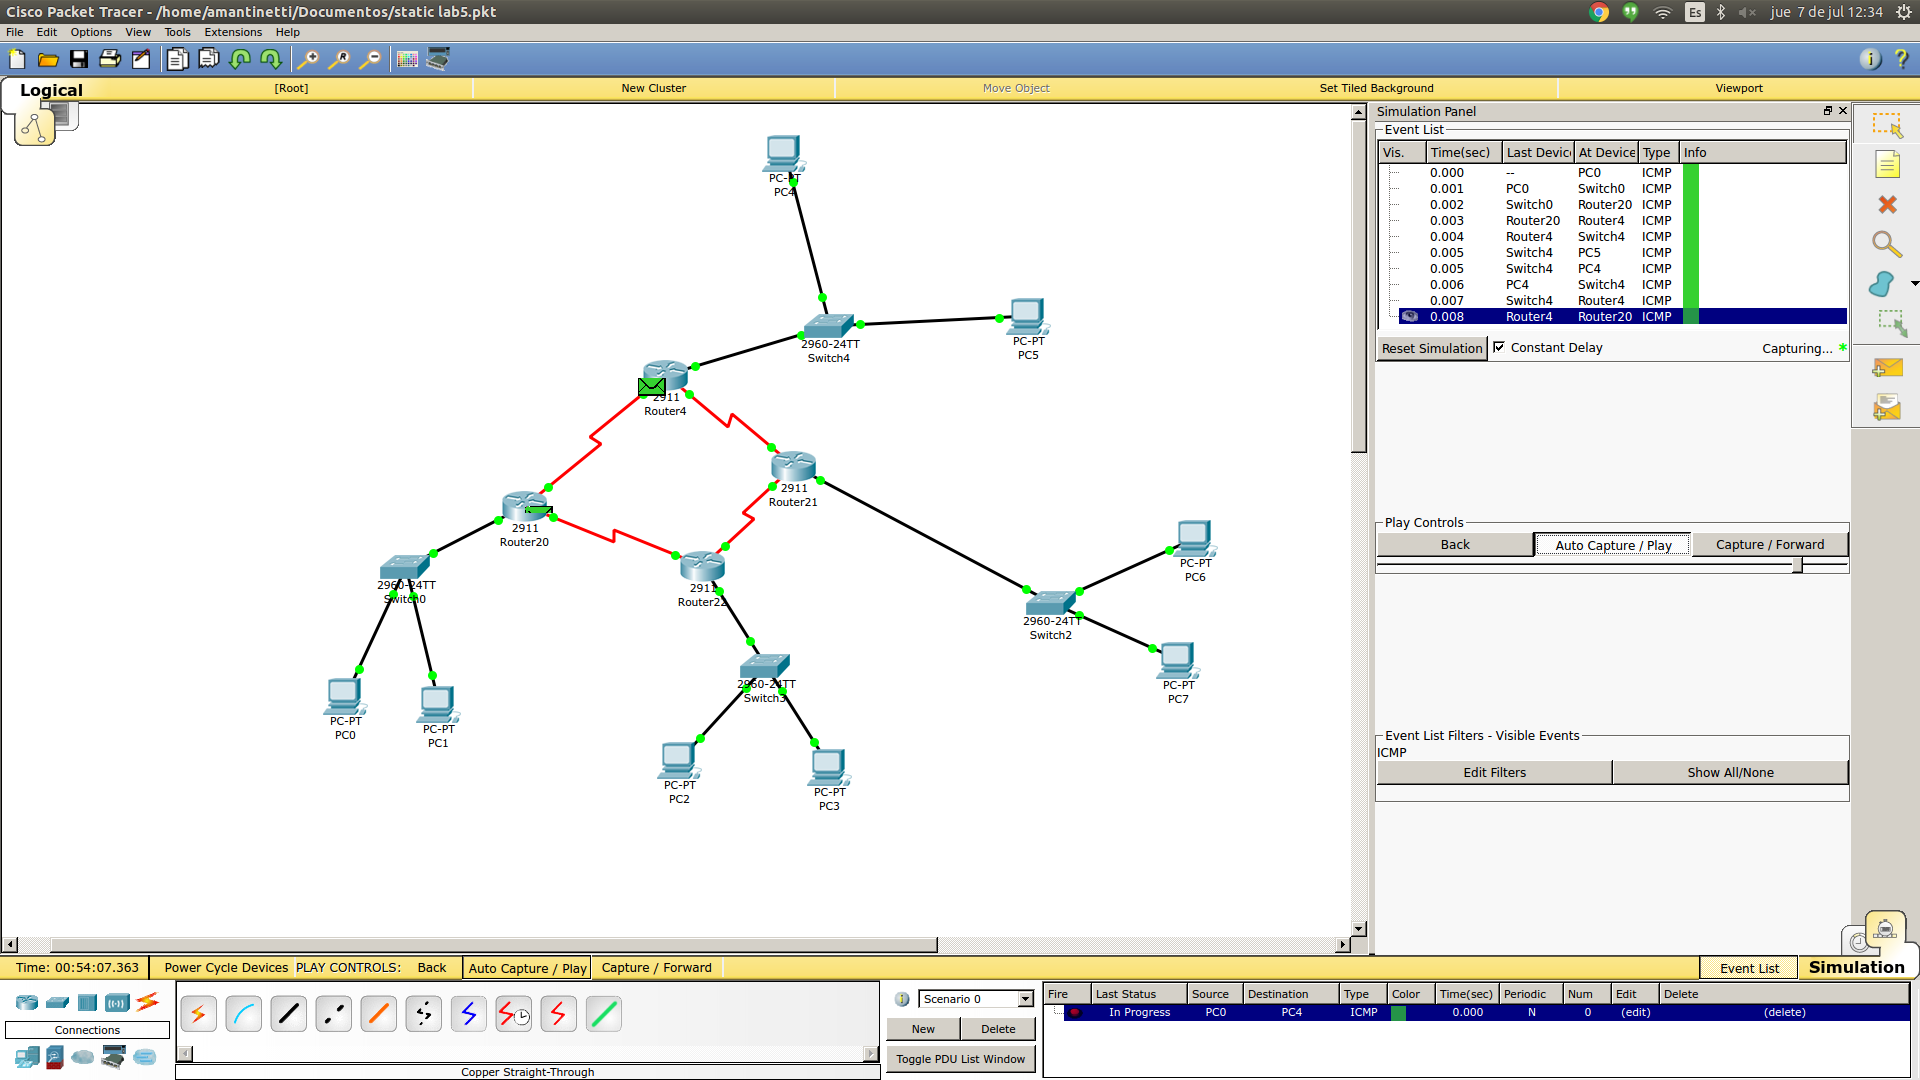
\includegraphics[scale=.25]{imagenes/test_rdinamic.png}
	\caption{Test Ruteo Dinámico}
	\label{fig:Figura 4.2}
\end{figure}

\subsection{¿Qué ventajas y desventajas se pueden apreciar en cada tipo de enrutamiento?}
\begin{table}[H]
\centering
\begin{tabular}{p{8cm}|p{8cm}}
\textbf{Enrutamiento Dinámico} & \textbf{Enrutamiento Estático} \\
     Se debe configurar el enrutamiento en cada router de la red &
     Los routers aprenden a enrutarse con los demas rourters de la red \\
     El rourter comparte su tabla de enrutamiento  & 
     El rourter NO comparte su tabla de enrutamiento  \\
     Los rourters tienen capacidad de modificar su enrutamiento en caso de fallo de red &
     Los rourters no tienen capacidad de reaccionar en caso de un fallo de red \\
     Utiliza mas CPU & 
     Minimiza el uso de CPU \\    
\end{tabular}
\end{table}

\subsection{¿En que se basa el enrutamiento dinámico para generar su ruta?}
El enrutamiento dinámico genera la ruta óptima en base a la información obtenida en tiempo real por algún protocolo de routing. Según el protocolo de ruteo, se pueden ocupar uno de dos algoritmos, vector distancia y estado de enlace. En el primero, cada router conoce la distancia de sus vecinos directamente conectados y les envía esta información. A su vez, estos le otorgarán la información sobre sus redes alcanzables y sus distancias. En el segundo, la distancia de un router y sus vecinos es enviada por broadcast a todos los routers de la red.



\listoffigures


\end{document}